\chapter{The Pin Column Model}
The flatland model of locks can explain effects that involve more than one pin, but a different model is needed to explain the detailed behavior of a single pin.
See Figure 5.1.
The pin-column model highlights the relationship between the torque applied and the amount of force needed to lift each pin.
It is essential that you understand this relationship.

In order to understand the "feel" of lock picking you need to know how the movement of a pin is effect by the torque applied by your torque wrench (tensioner) and the pressure applied by your pick.
A good way to represent this understanding is a graph that shows the minimum pressure needed to move a pin as a function of how far the pin has been displaced from its initial position.
The remainder of this chapter will derive that force graph from the pin-column model.

Figure 5.2 shows a single pin position after torque has been applied to the plug.
The forces acting of the driver pin are the friction from the sides, the spring contact force from above, and the contact force from the key pin below.
The amount of pressure you apply to the pick determines the contact force from below.
The spring force increases as the pins are pushed into the hull, but the increase is slight, so we will assume that the spring force is constant over the range of displacements we are interested in.
The pins will not move unless you apply enough pressure to overcome the spring force.
The binding friction is proportional to how hard the driver pin is being scissored between the plug and the hull, which in this case is proportional to the torque.
The more torque you apply to the plug, the harder it will be to move the pins.
To make a pin move, you need to apply a pressure that is greater than the sum of the spring and friction forces.

When the bottom of the driver pin reaches the sheer line, the situation suddenly changes.
See Figure 5.3. The friction binding force drops to zero and the plug rotates slightly (until some other pin binds).
Now the only resistance to motion is the spring force.
After the top of the key pin crosses the gap between the plug and the hull, a new contact force arises from the key pin striking the hull.
This force can be quite large, and it causes a peak in the amount of pressure needed to move a pin.

If the pins are pushed further into the hull, the key pin acquires a binding fiction like the driver pin had in the initial situation.
See Figure 5.4.
Thus, the amount of pressure needed to move the pins before and after the sheer line is about the same.
Increasing the torque increases the required pressure.
At the sheer line, the pressure increases dramatically due to the key pin hitting the hull.
This analysis is summarized graphically in Figure 5.5.

\begin{figure}
    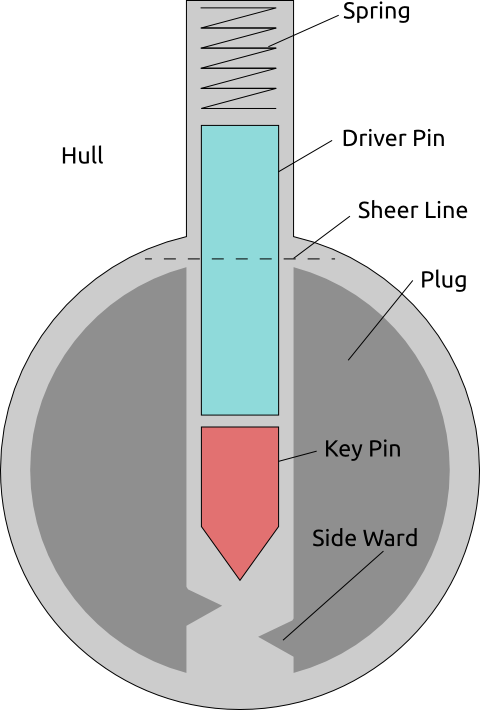
\includegraphics[scale=0.5]{figure5.1}
    \caption{The pin-column model}
\end{figure}

\begin{figure}
    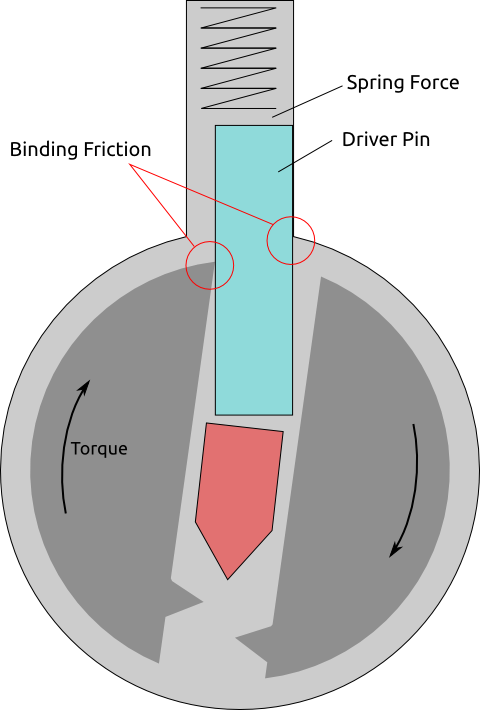
\includegraphics[scale=0.5]{figure5.2}
    \caption{Binding in the pin-column model}
\end{figure}

\begin{figure}
    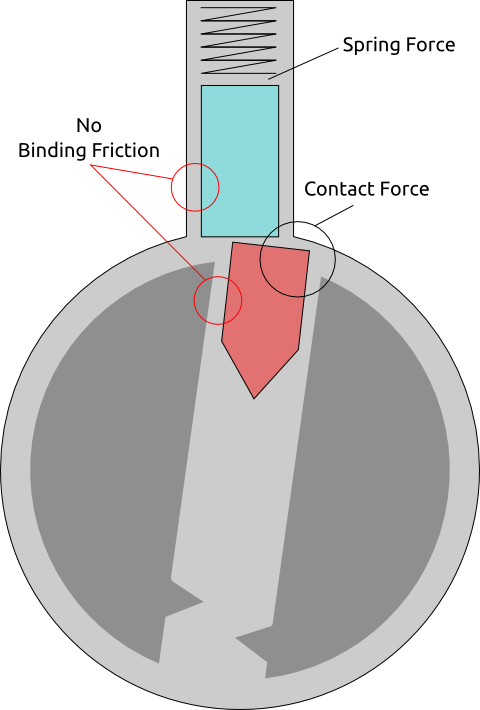
\includegraphics[scale=0.5]{figure5.3}
    \caption{Pins at the sheer line}
\end{figure}

\begin{figure}
    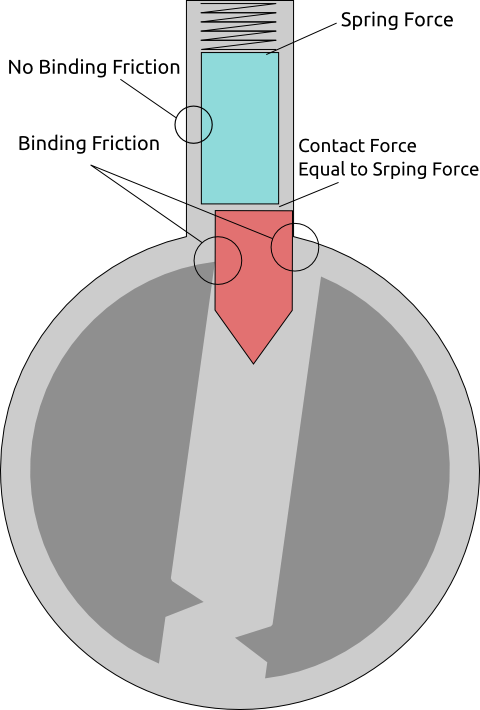
\includegraphics[scale=0.5]{figure5.4}
    \caption{Key pin enters hull}
\end{figure}

\begin{figure}
    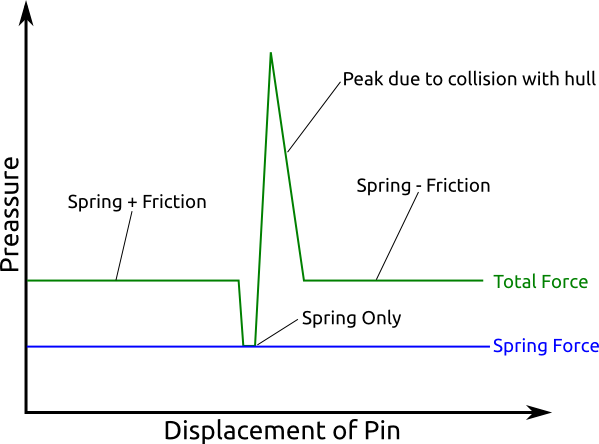
\includegraphics[width=\textwidth]{figure5.5}
    \caption{Pressure required to move pins}
\end{figure}
